\documentclass[11pt]{beamer}
\usepackage{verbatim}
\usetheme[progressbar=frametitle,numbering=fraction]{metropolis}
\usecolortheme{dove}

\usepackage{booktabs}
\usepackage[scale=2]{ccicons}
\usetikzlibrary{arrows,calc}
\usetikzlibrary{shapes}
\tikzstyle{line} = [draw, -latex']

\tikzstyle{block} = [rectangle, draw, fill=white, 
    text width=5em, text centered, rounded corners, minimum height=2em]

\tikzstyle{cloud} = [draw, ellipse,fill=white, node distance=3cm,
    minimum height=2em]
\usepackage{pgfplots}
\usepgfplotslibrary{dateplot}

\usepackage{xspace}
\newcommand{\themename}{\textbf{\textsc{metropolis}}\xspace}

\title{Marking protein coding boundaries on the genome using RNNs}
\subtitle{}
\date{\today}
\author{Saket Choudhary}
\institute{}
%\titlegraphic{\hfill\includegraphics[height=1.5cm]{logo}}

\begin{document}

\maketitle
\begin{frame}{Central Dogma of Biology}
\begin{figure}
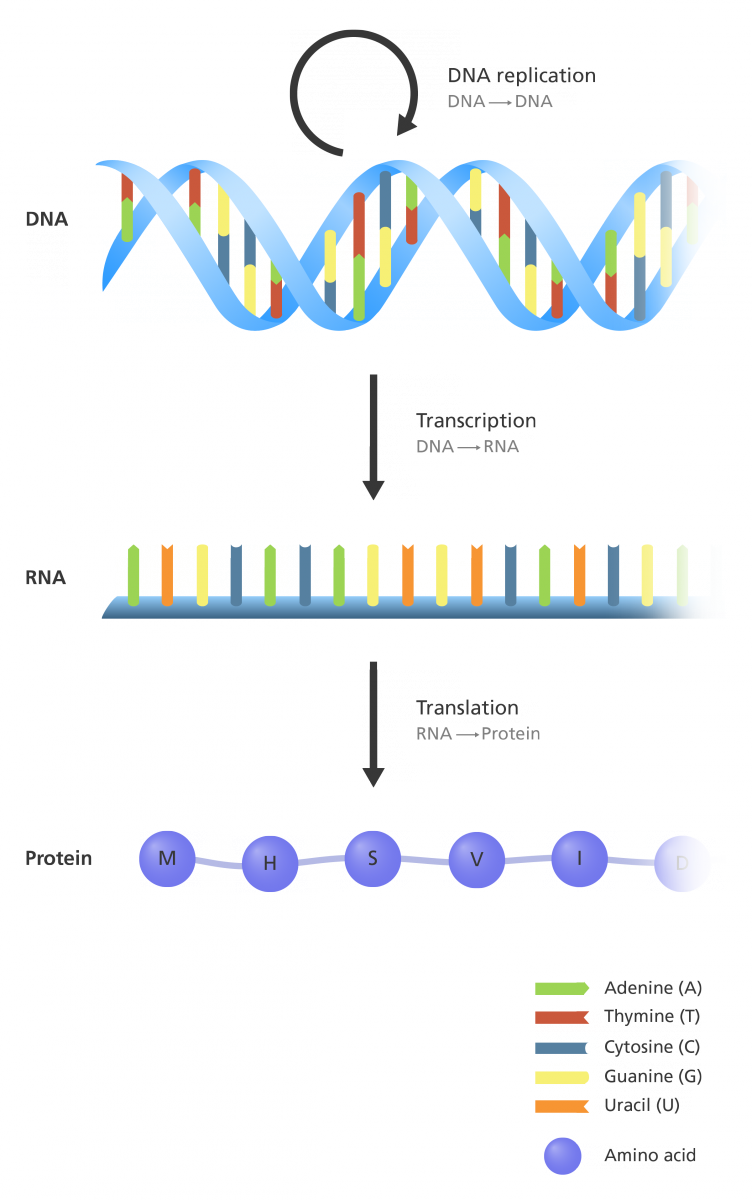
\includegraphics[width=\textwidth,height=\textheight,keepaspectratio]{central_dogma}
\end{figure}

\end{frame}

\begin{frame}{Gene clan be partitioned based on `coding' potential}
\begin{figure}
\includegraphics<1>[width=\linewidth]{MRNA_structure.png}
\includegraphics<2>[width=\linewidth]{distribution.png}
\end{figure}
\cite{calviello_beyond_2017}
\end{frame}

\begin{frame}{Motivation}
\begin{itemize}
\item `Close to exact' boundaries are known for a few organisms
\item Different partitions of the gene carry out different roles
\item Experiments require lot of resources and time!
\item Annotation is often required for any downstream application: for e.g. mutation analysis for personalized medicine
\end{itemize}
\end{frame}


\begin{frame}{Problem Formulation/Goal}
\textbf{Input}: A vector $\mathbf{x} \in \mathcal{V}^l$ where $l$ is sequence length  and $\mathcal{V} = \{N, A, C, T, G \}$. 

\textbf{Output}: Labels $\mathbf{y} = \{ \text{5'UTR}, \text{CDS}, \text{3'UTR} \}^l$

\end{frame}

\begin{comment}

\begin{frame}{Problem Formulation}
\begin{figure}
\includegraphics<1>[width=\linewidth]{MRNA_structure.png}
\includegraphics<2>[width=\linewidth]{distribution.png}
\end{figure}
\end{frame}
\end{comment}


\begin{comment}
\begin{frame}{Related Work}
\begin{itemize}
\item Translation ORF classifier \cite{chew_ribosome_2013} uses a random forest classifier
\item Implementation not public
\item Trained/tested on a single organism
\end{itemize}
\end{frame}
\end{comment}

\begin{frame}{Related Work: HMM based}
\begin{figure}
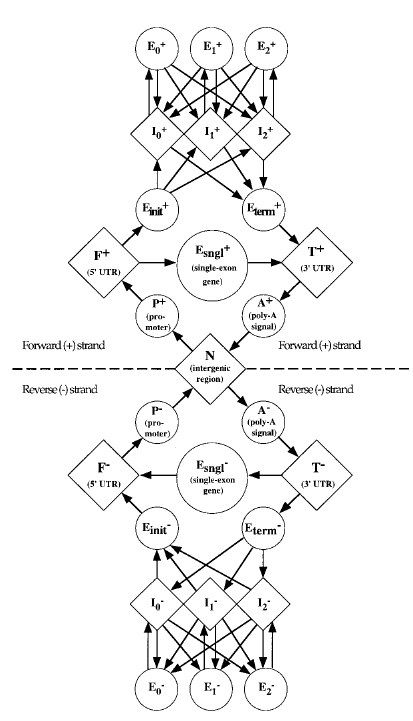
\includegraphics[width=\textwidth,height=0.8\textheight,keepaspectratio]{hmm_implementation}
\end{figure}
\cite{burge1997prediction}
\end{frame}

\begin{frame}{Data Availability}
National Center of Biotechnology Information - Sequence Read Archive(NCBI SRA) hosts genomic data from multiple organisms hosted publicly.

\url{https://www.ncbi.nlm.nih.gov/sra}
\begin{itemize}
\item Each organism has multiple genes. For example humans ~25000 genes with close to gold standard annotation
\item Around 7 more organisms with golden standard annotation
\end{itemize}


%\begin{figure}
%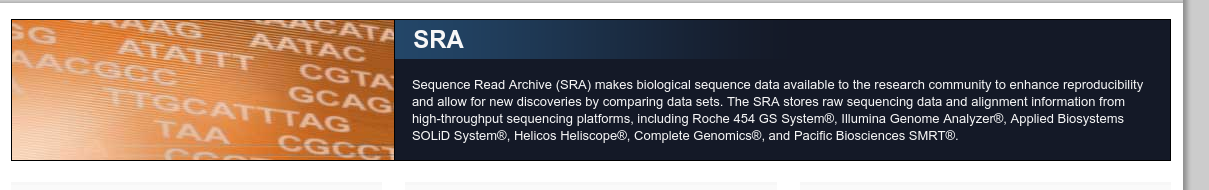
\includegraphics[width=\linewidth]{sra}
%\end{figure}

\end{frame}

\begin{frame}{Milestones}
\begin{enumerate}
\item Preprocessed datasets : Raw data $\Rightarrow$ Encoded
\item Minimal implementation : RNN
\item Within organism prediction : Well annotated genes in humans and mouse
\end{enumerate}
\end{frame}

\begin{comment}

\begin{frame}{Methods}
\begin{center}
Counts; annotation $\rightarrow$ RNN
\end{center}
\end{frame}
\end{comment}

\begin{frame}{Model/Results}
\begin{enumerate}
\item LSTM with sigmoid activation, 0.25 dropout
\item ~ 20000 genes with length 200 - 10,000 
\item Downsampled genes to 1000 first maintaining the length distribution
\item train:test = 70:30
\item 20 epochs so far
\end{enumerate}
\end{frame}

\begin{frame}{Preliminary results : Human (training)}
\begin{figure}
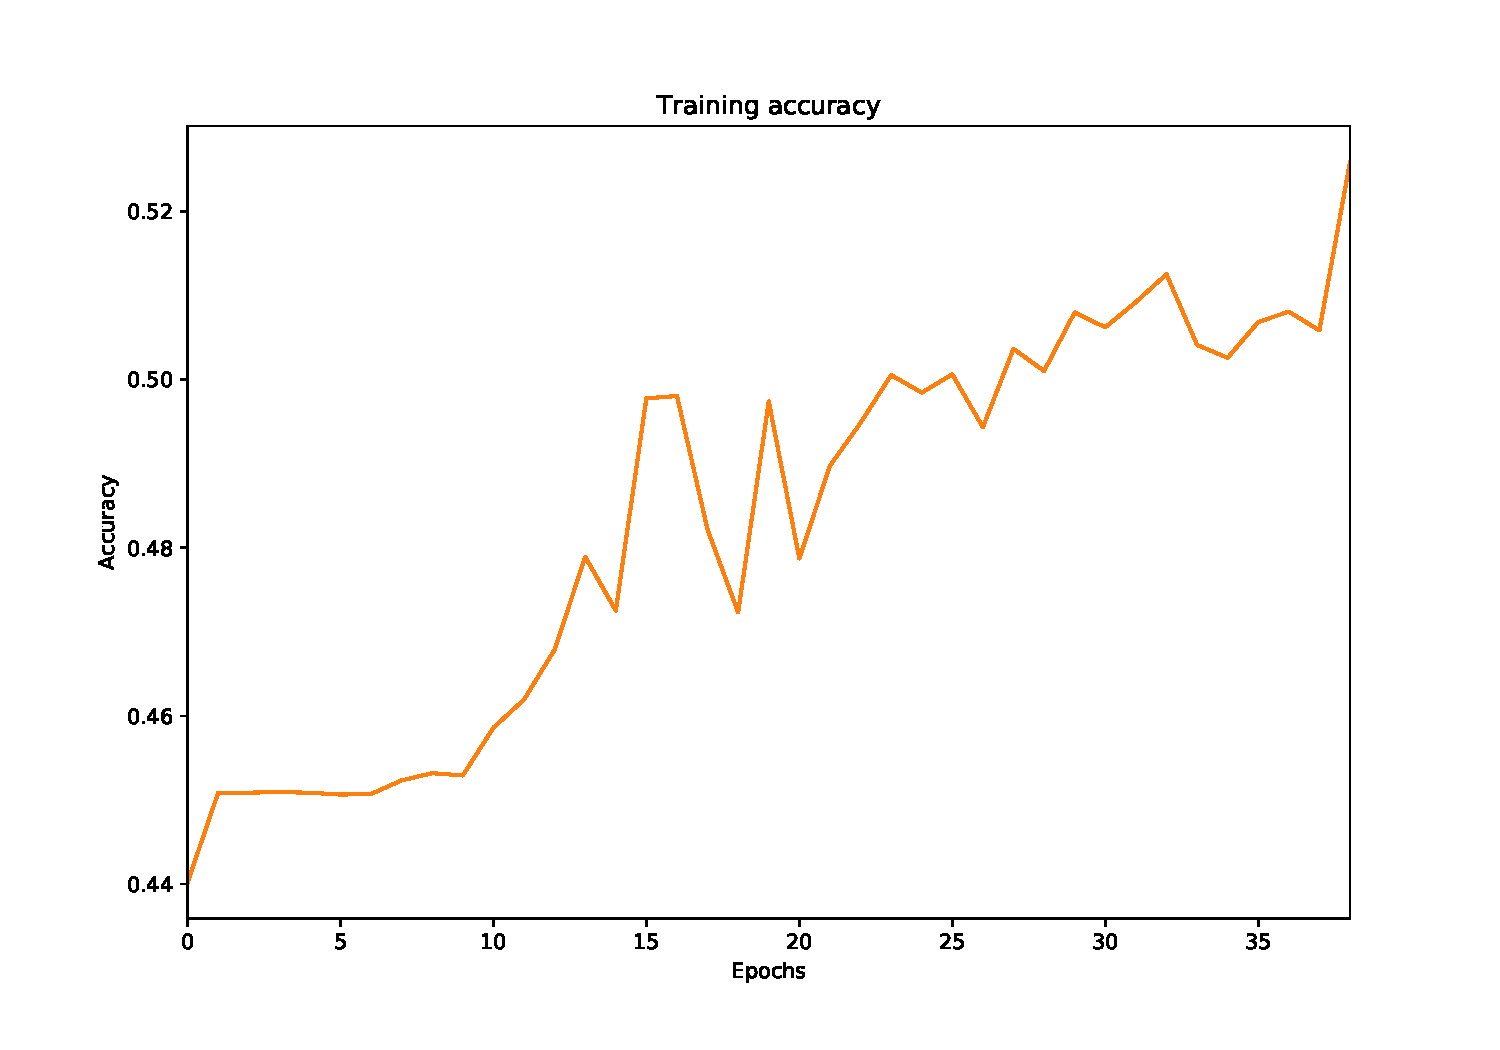
\includegraphics[width=\textwidth,height=\textheight,keepaspectratio]{training_accuracy_human}
\end{figure}
\end{frame}

\begin{frame}{Preliminary results : Human (testing)}
\begin{figure}
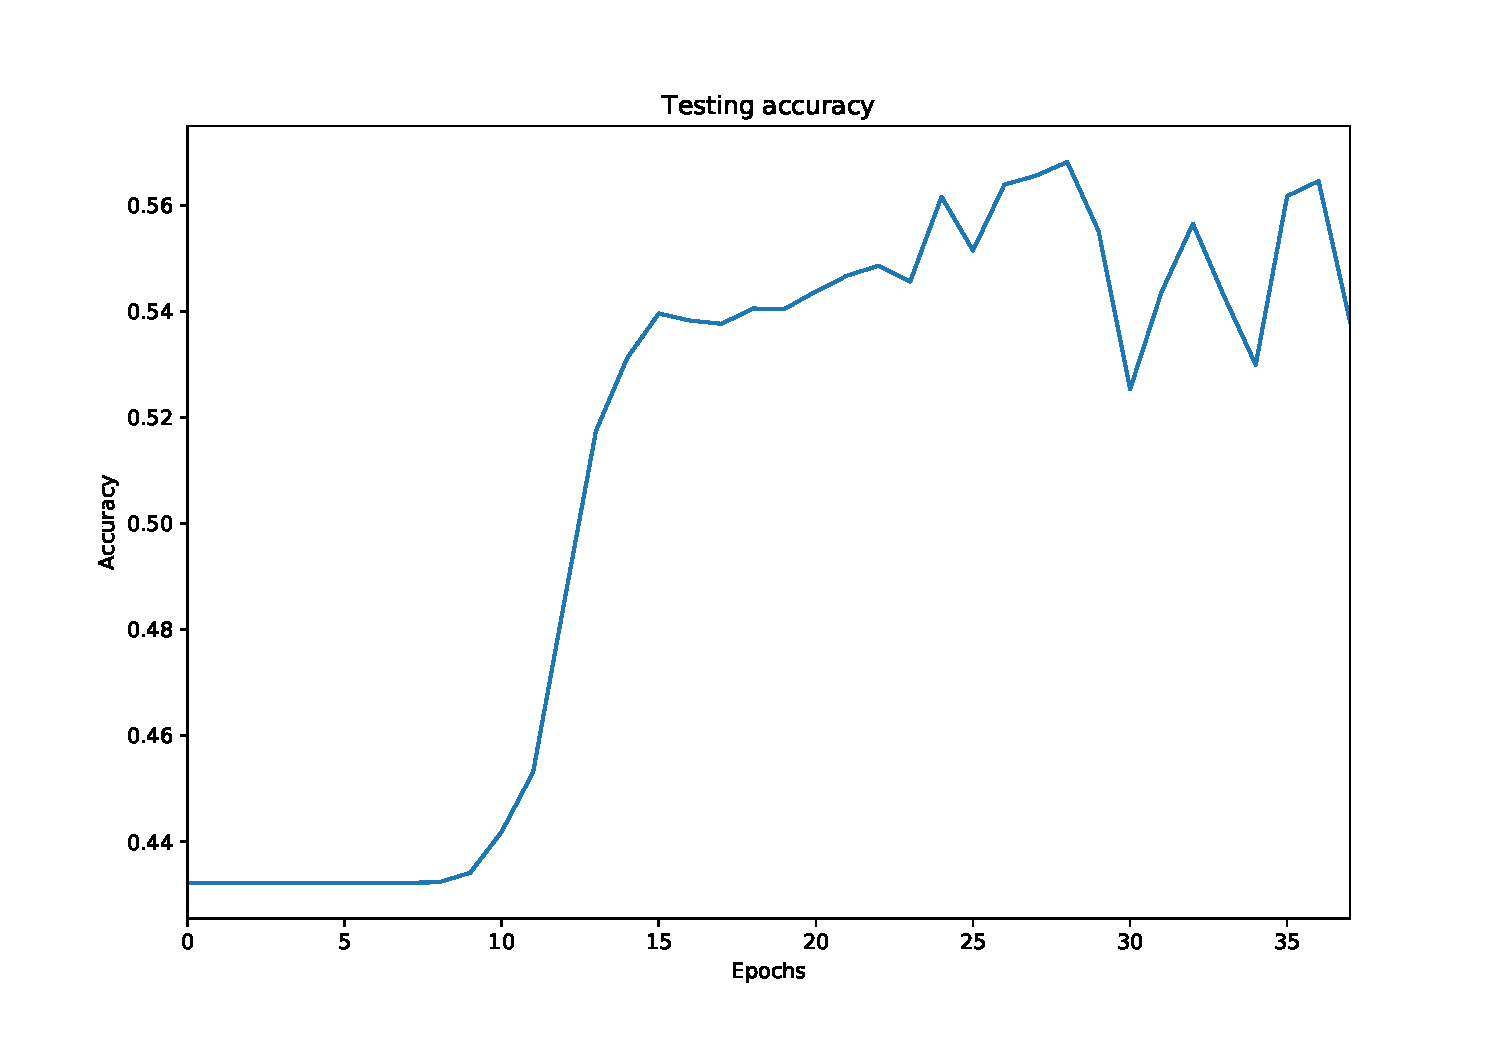
\includegraphics[width=\textwidth,height=\textheight,keepaspectratio]{testing_accuracy_human}
\end{figure}
\end{frame}

\begin{frame}{Preliminary results : Mouse (training)}
\begin{figure}
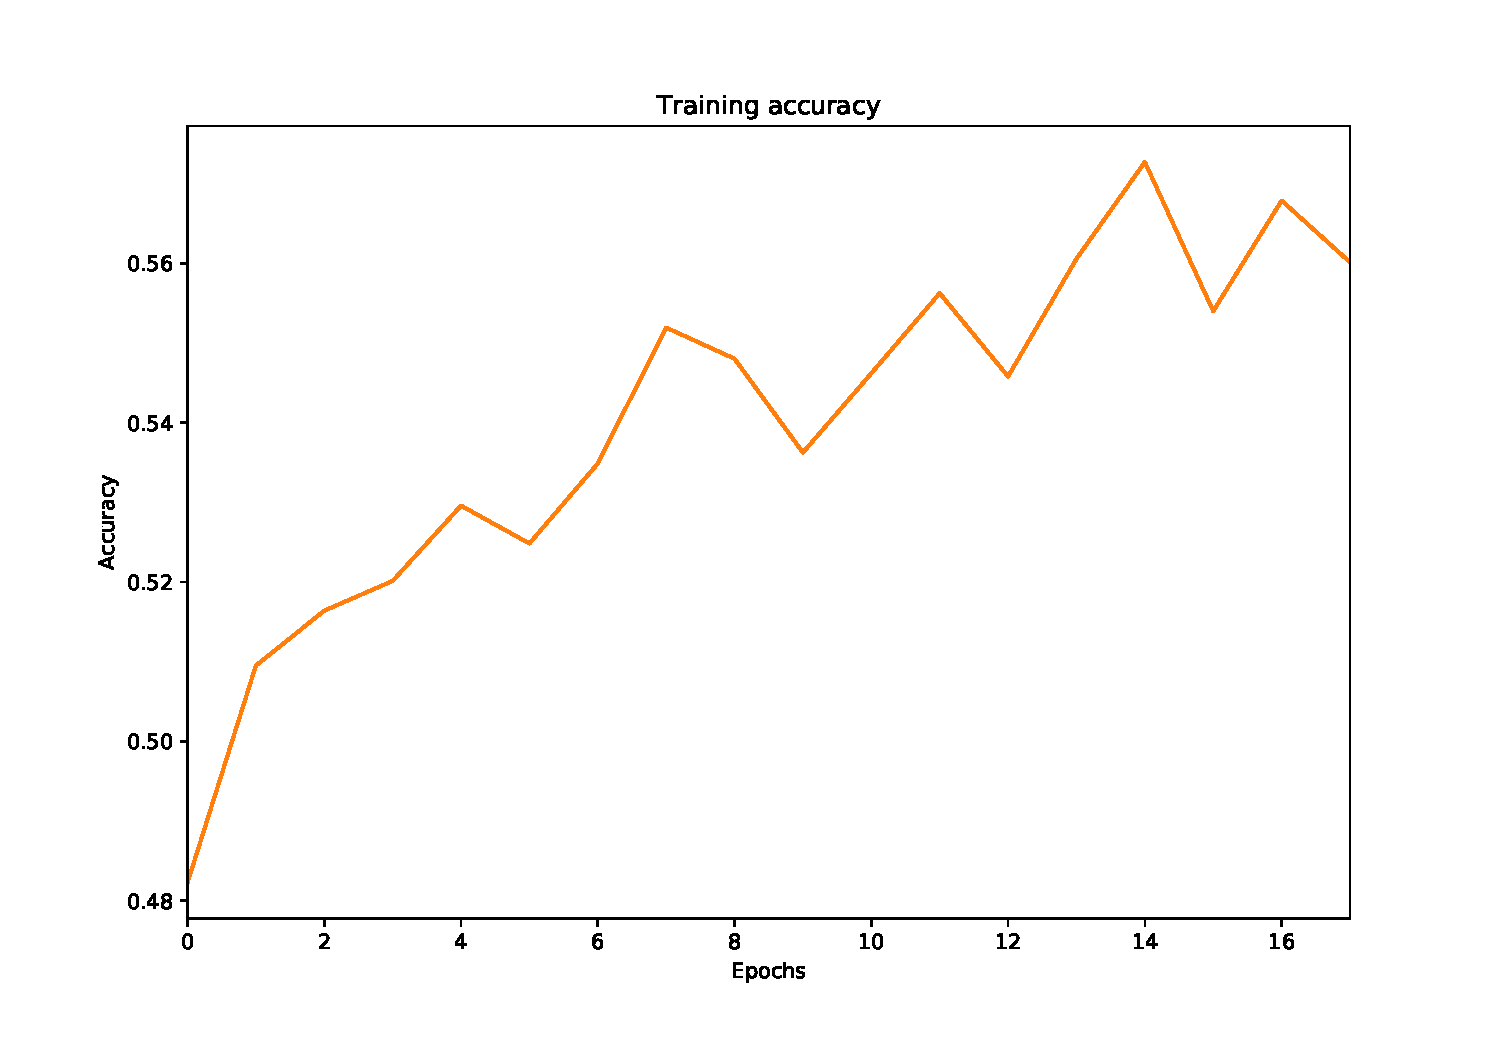
\includegraphics[width=\textwidth,height=\textheight,keepaspectratio]{training_accuracy_mouse}
\end{figure}
\end{frame}

\begin{frame}{Preliminary results : Mouse (testing)}
\begin{figure}
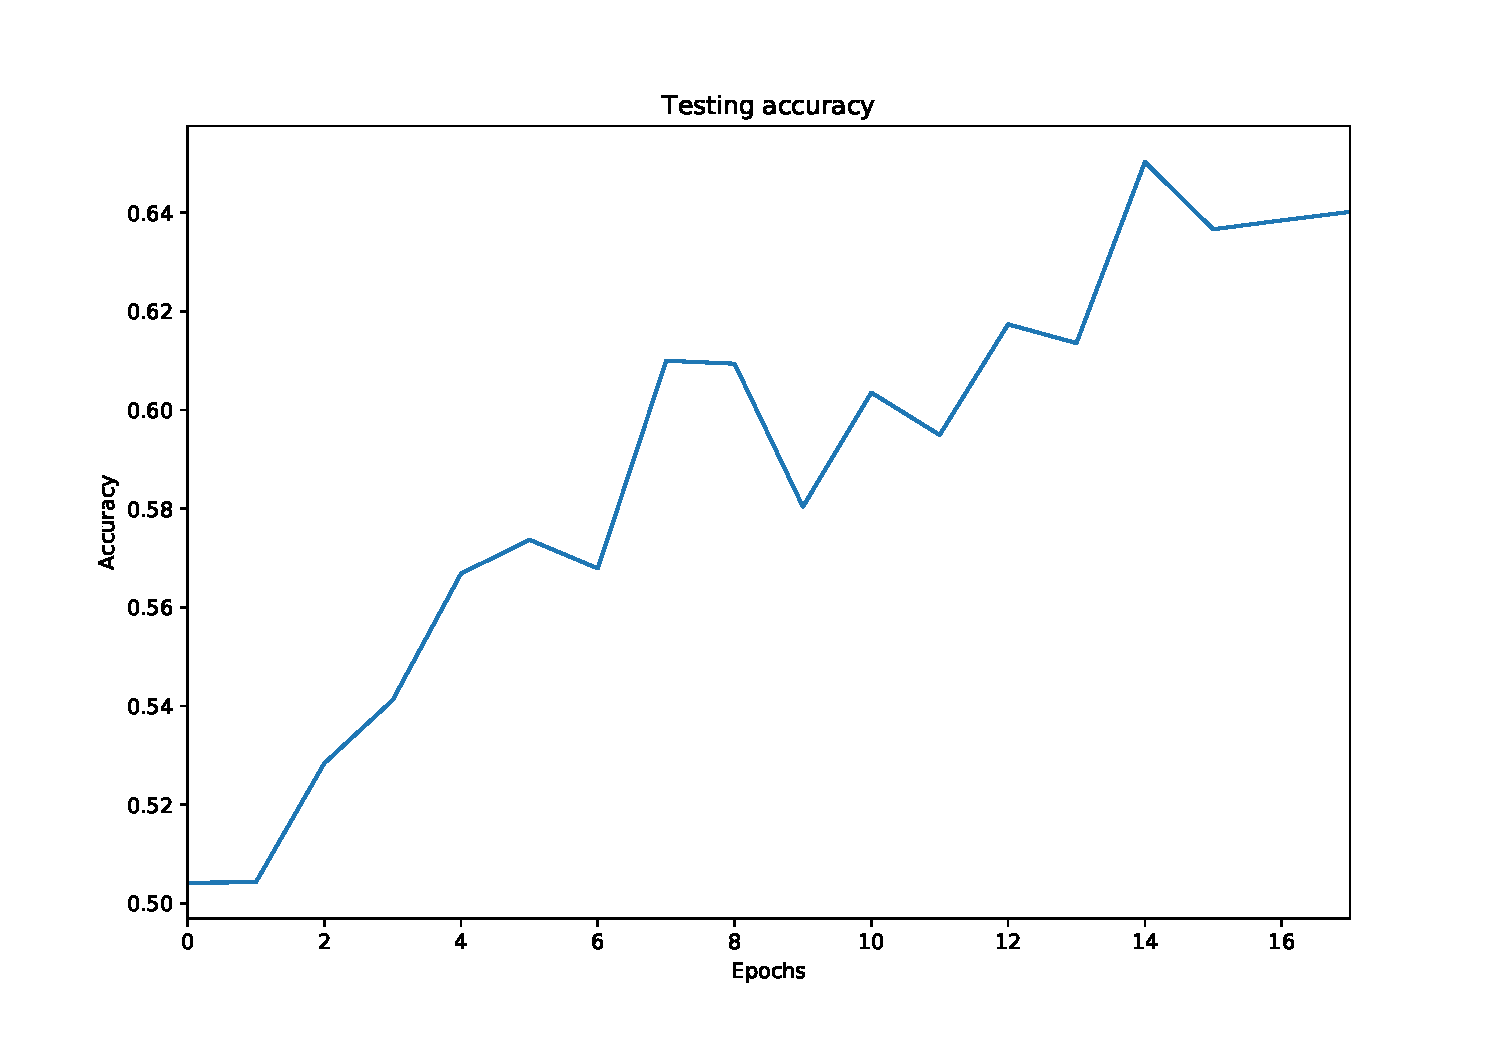
\includegraphics[width=\textwidth,height=\textheight,keepaspectratio]{testing_accuracy_mouse}
\end{figure}
\end{frame}



\begin{frame}{Plan}
\begin{enumerate}
\item Try with more epochs
\item Try increasing sample size
\end{enumerate}
\end{frame}

% \item Preprocessing is time consuming, requires uniformity across datasets

\begin{frame}[allowframebreaks]
        \frametitle{References}
        \bibliographystyle{apalike}
        \bibliography{main.bib}
\end{frame}

% \begin{frame}{Questions/Ideas}
% \begin{itemize}
% \item How has the binding site evolved across species?
% \item Coordinated evolutionary changes at various levels of gene regulation?
% \item Are transcription and post-transcription machinery coupled: do genes with complex regulatory system also have complex post-transcription? 
% \item Can TF occupancy be used to make predictions about RBP occupancy or vice versa? 
% %\item Quantifying Interplay between miRNA and RBPs
% \item RBPs in chromatin context: sites of integration? correlation between active marks and binding, relation to methylation?
% \item Can we use RBP binding information along with other assays(ChIP, open chromatin etc.) to make a model that can be used to infer gene regulation at different states, hierarchically.
% \end{itemize}

% \end{frame}

\end{document}
